\documentclass{article}

\usepackage[T1]{fontenc} % add special characters (e.g., umlaute)
\usepackage[utf8]{inputenc} % set utf-8 as default input encoding
\usepackage{ismir,amsmath,cite,url}
\usepackage{graphicx}
\usepackage{color}


\usepackage{lineno}
\linenumbers

% ------
\title{
Melody transcription via generative pre-training
%A fresh look at melody transcription
}

\threeauthors
  {First Author} {Affiliation1 \\ {\tt author1@ismir.edu}}
  {Second Author} {\bf Retain these fake authors in\\\bf submission to preserve the formatting}
  {Third Author} {Affiliation3 \\ {\tt author3@ismir.edu}}

% For the author list in the Creative Common license, please enter author names. 
% Please abbreviate the first names of authors and add 'and' between the second to last and last authors.
\def\authorname{F. Author, S. Author, and T. Author}

% Optional: To use hyperref, uncomment the following.
\usepackage[bookmarks=false,pdfauthor={\authorname},pdfsubject={\papersubject},hidelinks]{hyperref}
% Mind the bookmarks=false option; bookmarks are incompatible with ismir.sty.

\sloppy % please retain sloppy command for improved formatting

% My dependencies
\usepackage{booktabs}
\usepackage{cleveref}

% My macros
\newcommand{\madmom}{\texttt{madmom}}
\newcommand{\mel}{Mel}
\newcommand{\mtthree}{MT3}
\newcommand{\jukebox}{Jukebox}
\newcommand{\hooktheory}{HookTheory}
\newcommand{\rwc}{RWC-MDB}
\newcommand{\sheetsage}{Sheet Sage}

\begin{document}

\maketitle

\begin{abstract}
Melody 
%is among the most fundamental aspects 
is a fundamental aspect 
of 
%human 
music perception. 
%---even those without musical training can often recognize and reproduce melodies by ear. 
While even those without musical training can often recognize and reproduce melodies by ear, it remains an open challenge in MIR to transcribe an arbitrary recording of Western music into notes which constitute its melody. 
A key challenge in melody transcription is building methods which can handle broad audio containing any number of instrument ensembles and musical genres. 
To confront this challenge, we leverage recent advancements in generative modeling of broad music audio, thereby improving performance on melody transcription by up to $27$\% relative to conventional approaches. 
Another obstacle in melody transcription is a lack of training data---we collect, align, and release a new dataset consisting of $50$ hours of crowdsourced melody annotations for popular music. 
By pairing our new melody transcription approach with existing solutions for beat detection, key estimation, and chord recognition, 
we build the first system capable of transcribing human-readable lead sheets directly from music audio.\footnote{Sound examples: \url{https://dblblnd.github.io/ismir22} \\
Demo / dataset explorer: \url{https://colab.research.google.com/drive/1yzD3wRCjXkuSfDRUtt_daaGFitj5L88l}}
\end{abstract}


\section{Introduction}\label{sec:introduction}

In the Western music canon (and especially in popular music), 
\emph{melody} is a defining characteristic of musical composition. 
Even those without formal musical training can often effortlessly recognize a melody within a complex mixture of sounds, 
a ubiquitous skill which forms a pillar of our collective musical experience. %experience. 
Because of the significance of melody to music perception, 
the ability to automatically \emph{transcribe} an arbitrary recording into 
%equal-tempered notes which constitute its melody 
its melody notes 
could enable numerous applications in 
% TODO: performance?
interaction~\cite{ryynanen2008accompaniment}, 
education~\cite{droe2006music}, 
informatics~\cite{bainbridge1999towards}, 
retrieval~\cite{ghias1995query}, 
source separation~\cite{ewert2014score},
and even generation~\cite{hawthorne2019enabling}.
Despite the numerous potential benefits, 
reliable melody transcription remains an open challenge in MIR.
%it remains an open challenge in MIR to transcribe an arbitrary recording into equal-tempered notes which constitute its melody.

% Why is it difficult?
The relative lack of progress on melody transcription is perhaps counterintuitive when compared to the considerable progress on seemingly more difficult tasks like piano transcription~\cite{sigtia2016end,hawthorne2017onsets}.
%and chord recognition~\cite{humphrey2012rethinking,boulanger2013audio}. 
This circumstance stems from two primary factors. 
First, unlike in piano transcription, melody transcription involves operating on \emph{broad} audio mixtures from arbitrary instrument ensembles and genres. 
% CHRIS: I think the following is indeed a big reason that melody transcription is hard, but it doesn't map cleanly onto any of our contributions
%Second, unlike in chord recognition, melody transcription involves isolating the notes from a single instrument voice (recognized to be the melodic voice) within the mixture. 
%Second, melody transcription involves not only detecting notes but also identifying which of those notes constitutes the melody, which may require modeling the nuances of human music perception. 
Second, little training data exists for melody transcription, which particularly impedes the deep learning approaches central to recent improvements in other areas of music transcription. 
% CHRIS: This maps cleanly onto our contributions (standardized evaluation and new datasets), but may be too snarky for paragraph 2
%Finally, we argue that a historical focus on the important but disparate task of melody \emph{extraction}---detecting the time-varying fundamental frequency of the melody as opposed to its discrete notes---has led to a lack of work on transcription and systemic issues in evaluation.

\begin{figure}
    \centering
    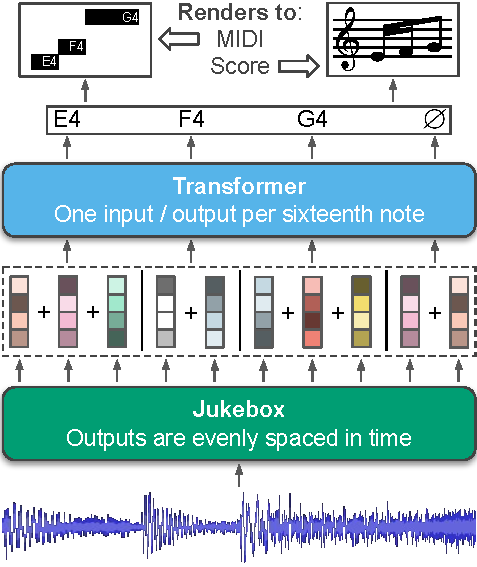
\includegraphics[width=8.1cm]{figs/fig1.pdf}
    \caption{
Our audio-to-score melody transcription approach involves 
(1)~extracting representations from Jukebox~\cite{dhariwal2020jukebox}, a generative model of music audio, 
(2)~averaging these representations across time to their nearest sixteenth note using \madmom~\cite{bock2016madmom,bock2016joint} for beat detection,
and
(3)~training a Transformer~\cite{vaswani2017attention} to detect melody note onsets (or rests) per sixteenth note.
}
 \label{fig:fig1}
\end{figure}

In order to overcome the challenge of transcribing broad audio, in this work we leverage representations from Jukebox~\cite{dhariwal2020jukebox}, a large-scale generative model of music audio pre-trained on $1$M songs~(\Cref{fig:fig1}). 
In~\cite{castellon2021calm}, Castellon~et~al.\ demonstrate that internal representations from Jukebox are useful for improving performance on a wide variety of MIR tasks. 
When used as input features to a Transformer~\cite{vaswani2017attention} model, representations from Jukebox outperform conventional spectrogram features used for melody transcription by 
% (RWC All) .744 vs .631 = 17.9%
% (Hookthr) .615 vs .514 = 19.6%
% (RWC Vox) .786 vs .621 = 26.6%
up to $27$\% relative. 
% CHRIS: This can be cut for space
To the best of our knowledge, this is the first evidence that representations from generative models of audio are useful for time-varying MIR tasks like transcription, as opposed to the song-level tasks (e.g.~genre detection) examined in~\cite{castellon2021calm}. 

To support this and future work on melody transcription, we collect and release a new dataset of crowdsourced melody annotations from the \hooktheory{} platform.\footnote{\url{https://www.hooktheory.com/theorytab}} 
This dataset contains $50$ hours of annotated melodies and harmonies (as chord names).  %and additionally contains chord labels.
%to aid chord recognition research. 
By training Transformer models on this new dataset using representations from Jukebox, we are able to improve overall performance on melody transcription by 
% 0.786 vs 0.462 = 70%
% 0.744 vs 0.420 = 77%
$77$\% 
compared to the strongest available baseline. 
While data from \hooktheory{} has been used previously for tasks like harmonization~\cite{chen2021surprisenet,yeh2021automatic}, chord recognition~\cite{jiang2019mirex}, and representation learning~\cite{jiang2020transformer}, making use of this platform for MIR is currently cumbersome and involves web scraping, reverse engineering a proprietary score format, and audio-to-score alignment. 
To ease this burden, we release all of the annotations in a simplified MIDI-like format under a Creative Commons license, with links and alignments to the audio on YouTube. 
We also release all code, models, and Docker containers needed for precisely reproducing all of our evaluations, enabling direct comparison in future work even as some audio inevitably disappears from YouTube.\footnote{Released upon publication}

\begin{figure*}
    \centering
    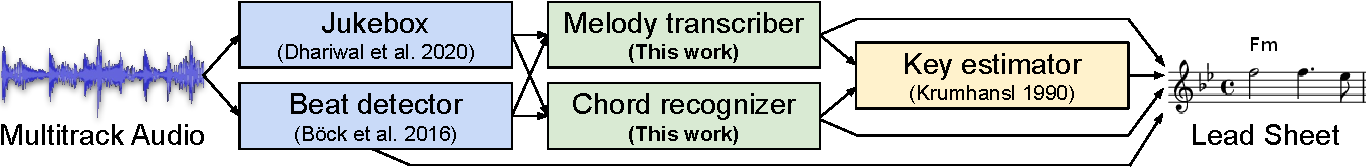
\includegraphics[width=\linewidth]{figs/sheet_sage.pdf}
    \caption{
    % TODO: Clean this up. YouTube as input
    Inference procedure for Sheet Sage, our proposed system which transcribes multitrack audio into lead sheets (scores which depict melody as notes and harmony as chord names). The blue, green, and yellow boxes respectively take audio, features, and symbolic music data as input. Green boxes are modules that we built as part of this work---both are Transformers~\cite{vaswani2017attention} trained on their respective tasks using audio features from Jukebox~\cite{dhariwal2020jukebox} and data from \hooktheory~\cite{hooktheory}.}
    \label{fig:sheet_sage}
\end{figure*}

We also propose a new strategy for training transcription models in the presence of imprecise alignments. 
User annotations from \hooktheory{} are aligned to the audio at the segment level. 
We use beat tracking to refine these alignments, but they are still not as precise as the flawless alignments found in other transcription datasets (e.g.,~piano transcription datasets captured using a Disklavier) which existing methods rely on. 
Our approach involves aggregating input features (evenly spaced in \emph{time}) into proxy features which represent individual sixteenth notes (evenly spaced in \emph{beats}), 
which effectively smooths over alignment jitter. 
This approach has a secondary benefit of trivializing the process of converting output from the transcription model into a human-readable score-like format. %which is simpler for musicians to interpret compared to MIDI.

Finally, enabled by our state-of-the-art melody transcription approach, we present \emph{\sheetsage}, a system capable of automatically transcribing Western music audio into \emph{lead sheets}. 
A lead sheet is a human-readable musical score depicting a song's melody as notes on a staff and its harmony as chord names. 
The combination of melody and harmony represents the essence of a piece of Western music, and as such, lead sheets are commonly used by experts to easily perform recognizable renditions of existing pieces. 
As part of \sheetsage, we additionally train a Transformer-based chord recognition model on \hooktheory{} data using input features from Jukebox. 
To produce lead sheets, we pair this chord recognition model with our best melody transcription model, beat detections from \madmom~\cite{bock2016madmom,bock2016joint}, key estimations from Melisma~\cite{krumhansl1990cognitive,temperley1999key,sleator2001melisma}, and engraving with LilyPond~\cite{nienhuys2003lilypond}~(\Cref{fig:sheet_sage}). 
By automatically transcribing music audio into lead sheets, our work helps reduce the gap between human perception and machine understanding of Western music.

\section{Related work}

% Melody extraction

\section{Task definition}


\begin{figure}
    \centering
    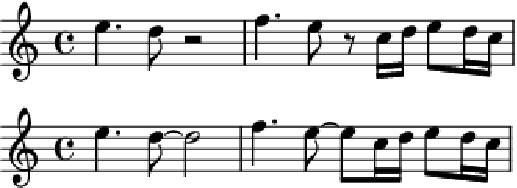
\includegraphics[width=8.1cm]{figs/heuristic_offsets.pdf}
    \caption{
The same note onsets engraved with ground truth~(top) vs. heuristic~(bottom) offsets. 
We argue that onset prediction suffices for producing human-readable melody transcriptions.
}
 \label{fig:heuristic_offsets}
\end{figure}

\section{Methods}

\section{Experiments}

\begin{table}[]
    \centering
    \begin{tabular}{lcc}
\toprule
Features & $d$ & Onset F1 \\
\midrule
\mel{} & $229$ & $0.514$ \\
\mtthree{} & $512$ & $0.550$ \\
\jukebox{} & $4800$ & $0.615$ \\
\mel{}, \mtthree{} & $741$ & $0.548$ \\
\mel{}, \jukebox{} & $5029$ & $0.617$ \\
\mtthree{}, \jukebox{} & $5312$ & $0.622$ \\
\mel{}, \mtthree{}, \jukebox{} & $5541$ & $\mathbf{0.623}$ \\
\bottomrule
    \end{tabular}
    \caption{\hooktheory{} test set performance of different combinations of representations (when passed as input to train a Transformer). Different representations do contain complimentary information---combining all three yields highest performance---but Jukebox on its own is competitive with all combinations.}
    \label{tab:hooktheory_test}
\end{table}

\begin{table}[]
    \centering
    \begin{tabular}{lcc}
\toprule
 & Onset F1 & Onset F1 \\
Approach & \emph{Vox Only} & \emph{All} \\
\midrule
MT3 Zero-shot~\cite{gardner2021mt3} & $0.085$ & $0.133$ \\
Melodia~\cite{salamon2014melody} + Segmentation & $0.268$ & $0.201$ \\
DSP + HMM~\cite{ryynanen2006transcription,ryynanen2008automatic} & $0.381$ & $0.420$ \\
Spleeter~\cite{hennequin2020spleeter} + Tony~\cite{mauch2015computer} & $0.462$ & $0.341$ \\
\midrule
\mel{} + Transformer & $0.621$ & $0.631$ \\
\mtthree{} + Transformer & $0.659$ & $0.701$ \\
\jukebox{} + Transformer & $\mathbf{0.786}$ & $\mathbf{0.744}$ \\
\bottomrule
    \end{tabular}
    \caption{Performance of different approaches on a small subset of \rwc~\cite{goto2002rwc,goto2003rwc,goto2004development}. The bottom three approaches were trained on the \hooktheory{} dataset as part of this work. We compute performance on both vocals and all melody instruments for fair comparison to baselines designed for vocal transcription.}
    \label{tab:rwc_ryy}
\end{table}

\section{Sheet Sage}

\section{Conclusion}


\bibliography{main}

\end{document}

